\section{Metrics, planar fillings, and torsion}
\label{sec:geometry-foundations}

We begin the proof of Theorem~\ref{thm:triangle-complex}. Here we establish
two conclusions: nonempty closed edge paths with cyclic
turns of link distance at least $\pi$ are nontrivial, and $\pi_1(K)$ is
torsion-free. Reduced planar fillings turn angular-link bounds into a
curvature obstruction; shortest free loops turn that obstruction into
torsion-freeness. Uniform thinness and the passage to the Cayley graph
are proved in Section~\ref{sec:geometry-thinness}.

Throughout this section, $K$ is the finite Euclidean triangle complex in that theorem;
``original'' refers to its cells before subdivision. A link is regarded as a
metric graph, with the length of each edge equal to the angle of its corner.
As in Section~\ref{sec:construction}, a closed link walk is
\emph{cyclically reduced} if consecutive edges, including the last
and first, are never mutual reverses.

\subsection{Subdivisions and shortest paths}

Barycentrically subdivide $K$. This gives a genuine simplicial complex:
its vertices are the original cells, and its simplices are their strict
inclusion chains. In particular, distinct parallel original edges have
distinct barycenters, and triangles meeting in several faces cause no
identifications within a simplex. Realize the subdivision by straight
segments in each Euclidean triangle. At an original vertex this only
subdivides the angular link, preserving its metric. At a point in the
interior of an original triangle, the link is a circle of length $2\pi$.
At a point in the interior of an original edge, its two tangent directions
are joined by one path of length $\pi$ for each incident triangle. If there
are no incident triangles, the two directions are isolated. Thus every
nonempty cyclically reduced closed walk at a new vertex has length
at least $2\pi$; at an original vertex the stronger lower bound
$2\pi+\eta$ remains valid.

These statements hold after any further compatible Euclidean subdivision.
For the later uniform estimates we will return to the fixed barycentric
subdivision, in which each small triangle has an original vertex among its
vertices.

The intrinsic distance on a connected finite Euclidean triangle complex
is the infimum of the lengths of finite paths made of straight segments
in its cells. We use the same convention on the planar complexes below,
which may have edges belonging to no triangle and pieces meeting only at
a vertex.

\begin{lemma}[Metric preliminaries]
\label{lem:finite-geodesics}
This intrinsic distance is a metric inducing the complex topology. The
complex is compact, any two points are joined by a shortest path, and every
constant-speed local geodesic has finitely many straight pieces on a compact
parameter interval. The last assertion also holds for closed local geodesics.
If such a path lies in the edges of a Euclidean subdivision, the link
distance at each of its turns is at least $\pi$.
\end{lemma}

\begin{proof}
At a point $x$, cut the incident cells into sectors centered at $x$ and
choose $\rho>0$ smaller than the distances to their nonincident faces.
The resulting truncated star consists of finitely many sectors and,
possibly, isolated radial intervals, glued along radial sides. Its radial
coordinate $r$ agrees across these gluings, and changes by at most the
length of a polygonal path. In particular, a path from $x$ leaving the
star has length at least $\rho$. For a point of radius $r<\rho$, the radial
segment has length $r$; any shorter competitor stays in the star and has
length at least $r$. Hence its distance from $x$ is exactly $r$.

This description proves positivity of the distance and identifies the
small metric neighborhoods with the usual star neighborhoods. The metric
therefore induces the complex topology. It also supplies contracting
neighborhoods, by radial contraction. Finiteness of the complex gives
compactness. Parameterize a sequence of polygonal paths whose lengths
decrease to the distance between two fixed points proportionally to
arclength on $[0,1]$. Their speeds are uniformly bounded. Compactness and
equicontinuity give a uniformly convergent subsequence: this follows, for
example, by a diagonal choice on a countable dense subset of $[0,1]$ and
then the common modulus of continuity. For every fixed partition, the
sum of distances between successive points passes to the limit. Taking
the supremum over partitions shows that the limiting path has length at
most the limiting lengths. Since every path has length at least the
distance of its endpoints, this is a shortest path.

Consider now a sufficiently short unit-speed minimizing arc starting at
$x$. Its image lies in the truncated star, and the preceding radial
formula gives $r(t)=t$. At positive radius, its direction varies
continuously in the finite graph of directions of the star. If that
direction were nonconstant, it would traverse an interval in the interior
of one of the graph's edges: a continuous map with image in the finite
set of junctions and isolated directions is constant. Choose a subarc
inside the corresponding open sector whose endpoint directions differ.
The sector is locally Euclidean, and the length of this subarc is at
least the Euclidean distance of its endpoints, which is strictly larger
than the difference of their radii. This contradicts $r(t)=t$ and
unit speed. Thus the arc is radial and straight in one sector or radial
edge. Apply the argument on both sides of each parameter value of a local
geodesic. A finite subcover of its compact parameter interval gives
finitely many straight pieces. For a closed curve use the parameter
circle, so this also includes its seam.

Finally, an angular path of length less than $\pi$ between the incoming
backward direction and the outgoing direction yields a shorter chord.
Indeed, take two nearby points at equal distance from the turn, unfold
the consecutive sectors traversed by that angular path, and join the
points by the straight chord in the sector of total angle less than
$\pi$. Its length is less than the sum of the two radial lengths.
The chord maps back to a path in the complex; the unfolded sector need
not be embedded there. This contradicts local minimality.
\end{proof}

\subsection{Reduced planar fillings with a prescribed boundary}

A \emph{planar diagram} will mean a finite connected complex embedded
topologically in the plane, with edges and triangular faces, such that
every bounded complementary face of its graph is filled by a triangle.
Its exterior walk goes once around the unbounded complementary face,
counting incidences: it can repeat vertices, and traverses an edge with
no incident triangle twice. The embedding specifies the cyclic orders;
the Euclidean metrics on the triangles need not come from this planar
embedding.

\begin{lemma}[Reduced fillings]
\label{lem:reduced-diagrams}
Let $S$ be the barycentric subdivision of $K$, or a further compatible
Euclidean simplicial subdivision. Every prescribed nonempty
nullhomotopic closed edge path in $S$ is the exterior walk of a planar
diagram $\Delta$ with a map $\Delta\to S$ that maps each edge and triangle
isometrically onto an edge and triangle, respectively. Each triangle of
$\Delta$ has three distinct vertices and edges. At every interior
vertex of $\Delta$, the cyclic sequence of corners maps to a nonempty
cyclically reduced closed walk in the target link.
Every edge loop in $\Delta$ contracts in $\Delta$.
\end{lemma}

\begin{proof}
We form a labelled picture from a disk filling, minimize its number of
nodes, erase components disjoint from the boundary, and take the planar
dual, retaining the prescribed boundary word, including spurs.
Start with a continuous filling of the path by a disk,
with its boundary mapped linearly along each prescribed edge traversal.
Mark all boundary breakpoints. Barycentric coordinates for the vertices
of the genuine simplicial complex $S$, extended by zero outside their
stars, are continuous. Triangulate the disk sufficiently finely,
respecting the marked boundary points, that each coordinate varies by
less than $1/4$ on each domain triangle. Label a domain vertex by a
target vertex of largest coordinate in its image. This coordinate is
at least $1/3$, because $S$ has dimension at most two. At every point of
a domain triangle all its chosen labels therefore have positive
coordinate, since $1/3-1/4>0$. They belong to one target simplex.
Extending the labels linearly gives a simplicial map, allowing collapsed
edges and triangles.

Along each prescribed boundary edge the only possible labels are its
two endpoints. The boundary parametrization is monotone along that edge,
so the largest-coordinate label changes from the initial endpoint to the
terminal endpoint exactly once; either choice at a midpoint tie has this
property. Consequently the noncollapsed boundary steps are exactly the
prescribed edge word, in its prescribed order. The same argument on an
interval or circle shows that every loop based at a vertex has a based
edge-loop representative: the original map and its approximation
interpolate inside common target simplices, fixing the basepoint.

For the simplicial filling, draw the inverse images of ties for the
largest target coordinate. Inside a domain triangle mapped onto a
target triangle they are three arcs meeting at a trivalent node.
Inside a triangle mapped to an edge they form one separating arc, and
inside a triangle mapped to a vertex they are absent. Suppress all bends
of valence two. We obtain a finite polygonal \emph{picture}: its regions
are labelled by target vertices; an arc separates distinct labels that
span a target edge; and the three labels at every interior trivalent
node span a target triangle. Its boundary endpoints are leaves, one for
each letter of the prescribed edge word. Components disjoint from the
boundary, including circles, are allowed.

Among all labelled pictures with these local rules and these boundary
data, choose one with the fewest trivalent nodes. No arc can join two
nodes labelled by the same target triangle. To see this, let the labels
on its two sides be $a,b$, and let $d$ be the third vertex of that
triangle. The selected arc and its endpoints form an embedded interval.
A sufficiently thin regular neighborhood is a disk meeting the four
other incident half-arcs in four distinct boundary slots
(Figure~\ref{fig:picture-cancellation}). The two slots
on the $a$-side both separate $a$ from $d$; those on the $b$-side both
separate $b$ from $d$. Erase the two nodes and the intervening arc and
join each of these two pairs along its side of the neighborhood, with
label $d$ between the new arcs. The new arcs do not cross, and every
boundary label of the neighborhood is unchanged. This gives a picture
with two fewer nodes.

The argument is unaffected if some of the four half-arcs reconnect
outside the neighborhood: their slots remain distinct and their outside
continuations retain the same labels. In particular, an additional arc
between the nodes merely makes a lens outside the chosen neighborhood.
An arc cannot join a node to itself, since the three incident arcs there
have three different target-edge labels.

\begin{figure}[htbp]
\centering
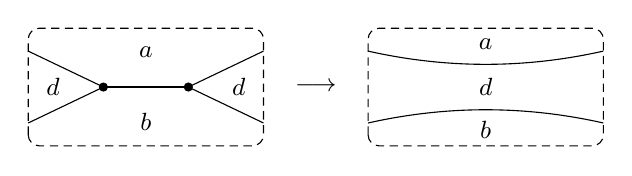
\begin{tikzpicture}[scale=.83, every node/.style={font=\small}]
  \begin{scope}[xshift=-2.6cm]
    \draw[densely dashed, rounded corners=4pt] (-1.8,-.9) rectangle (1.8,.9);
    \draw (-1.8,.55)--(-.65,0)--(-1.8,-.55);
    \draw (1.8,.55)--(.65,0)--(1.8,-.55);
    \draw (-.65,0)--(.65,0);
    \fill (-.65,0) circle (2pt);
    \fill (.65,0) circle (2pt);
    \node at (0,.53) {$a$};
    \node at (0,-.53) {$b$};
    \node at (-1.42,0) {$d$};
    \node at (1.42,0) {$d$};
  \end{scope}
  \node at (0,0) {$\longrightarrow$};
  \begin{scope}[xshift=2.6cm]
    \draw[densely dashed, rounded corners=4pt] (-1.8,-.9) rectangle (1.8,.9);
    \draw (-1.8,.55) .. controls (-.6,.28) and (.6,.28) .. (1.8,.55);
    \draw (-1.8,-.55) .. controls (-.6,-.28) and (.6,-.28) .. (1.8,-.55);
    \node at (0,.65) {$a$};
    \node at (0,-.65) {$b$};
    \node at (0,0) {$d$};
  \end{scope}
\end{tikzpicture}
\caption{Cancellation inside a thin disk neighborhood. Its four slots
and all boundary labels are preserved, regardless of reconnections
outside the disk.}
\label{fig:picture-cancellation}
\end{figure}

Next erase every component of the picture that misses the boundary.
Here the existence of consistent region labels deserves attention.
The retained picture together with the boundary circle is a connected
polygonal graph $H$. Each of its inside regions is a disk interior whose
boundary is a walk, possibly with repeated vertices and edges. One way
to see this is to build $H$ from the boundary circle: first attach tree
edges reaching all its other vertices, which slit disk regions, and then
add the remaining arcs, each of which splits a disk region into two.
Cutting apart repeated boundary incidences gives a polygon for each
region, with its interior embedded in the original disk.

Take a thin regular neighborhood of $H$ missing all erased components,
which are finitely many compact sets disjoint from $H$. For each inside
region, one connected curve in the boundary of this neighborhood follows
its entire boundary walk on the region side. In particular it follows
the two sides of a bridge separately, and follows every incidence at a
repeated vertex. This curve crosses no arc of the old picture and so lies
in one old labelled region. All labels prescribed along the boundary
incidences of the retained region are therefore equal. Extend that label
over the region. Erasing these components cannot increase the number of nodes,
so minimality is preserved.

Now construct its dual. Put a vertex in each region, and in that
region's polygon join this vertex to the midpoint of each incident arc
side by radii disjoint except at the vertex. Join the radii across the
arcs to obtain dual edges. Around each trivalent node the three
consecutive pairs of radii enclose a triangular region. Its three dual
vertices are distinct, since their region labels are the three distinct
vertices of a target triangle. The dual graph is connected, as can be
seen by taking paths between regions transverse to the picture arcs.

An Euler count verifies that these triangles fill all its bounded
faces. Let $E,N,L$ denote the numbers of retained picture arcs, trivalent
nodes, and boundary leaves. The boundary word is nonempty, so $L>0$.
Adjoining the circle subdivided at the leaves gives a connected planar
graph with $N+L$ vertices and $E+L$ edges. If $F$ is its number of inside
regions, Euler's formula gives
\[
 (N+L)-(E+L)+(F+1)=2,
 \qquad F=E-N+1.
\]
The dual graph has $F$ vertices and $E$ edges, hence exactly
$E-F+1=N$ bounded complementary faces. The $N$ disjoint triangular
regions already constructed exhaust them. Filling these triangles gives
the required planar diagram with no holes. The labels define its map
to $S$; assign each edge and triangle the metric of its image.

At a boundary leaf of the picture, its dual edge has an exterior
incidence. The interval between two successive leaves identifies the
corresponding sector at a region vertex. Following the original boundary
circle thus follows the dual exterior walk in exactly the prescribed
order. In particular, a picture arc with both endpoints on the boundary
produces an edge with no incident triangle, encountered twice. If there
are no nodes, the dual has $E+1$ vertices and $E$ edges and is a tree;
its spurs are still part of the exterior walk.

At an interior dual vertex, an immediate reversal of two successive
link edges would mean that the corresponding adjacent triangles map
to the same target triangle. Their picture nodes are joined by the
arc dual to their shared edge, contradicting minimality. This includes
the last and first corners in the cyclic order. Finally, every simple
edge circuit in the diagram bounds its filled planar disk. Any closed
edge walk splits at repeated vertices into such circuits and cancellable
backtracks, so every edge loop is nullhomotopic in the diagram.
\end{proof}

\subsection{Angular curvature and nontrivial closed paths}

Reduced fillings now let us compare the angular length of a target link
walk with the angles around a diagram vertex. Summing these angles will
show that a nullhomotopic boundary cannot have all its cyclic turns at
least $\pi$.

For a vertex $y$ of a diagram from Lemma~\ref{lem:reduced-diagrams}, let
$\theta_y$ be the sum of its incident triangle angles and let $n_y$ be
the number of exterior sectors there, equivalently its number of visits
in the exterior walk. Thus $n_y=0$ at an interior vertex. The reduced
link condition and the subdivision observations give
\[
 \theta_y\ge 2\pi \quad(n_y=0),\qquad
 \theta_y\ge 2\pi+\eta
 \quad\text{if also $y$ maps to an original vertex of $K$.}
\]

If $v,e,t$ count the vertices, edges, and triangles, planarity without
holes gives $v-e+t=1$. Counting exterior edge incidences, including both
sides of an edge belonging to no triangle, gives
$\sum_y n_y=2e-3t$. As each triangle has angle sum $\pi$, it follows that
\begin{equation}
 \sum_y\bigl((2-n_y)\pi-\theta_y\bigr)
 =2\pi v-\pi(2e-3t)-\pi t
 =2\pi.
 \label{eq:gauss-bonnet}
\end{equation}
This angular Gauss--Bonnet identity counts exterior visits with
multiplicity; it does not require a simple boundary.

\pagebreak[0]
\begin{samepage}
\begin{proposition}[Closed paths]
\label{prop:closed-paths}
In $K$, or any compatible Euclidean simplicial subdivision of it, a
nonempty closed edge path whose every cyclic turn has link distance at
least $\pi$ is not nullhomotopic.
\end{proposition}
\end{samepage}

\begin{proof}
First work in a simplicial subdivision and suppose such a path were
nullhomotopic. Apply Lemma~\ref{lem:reduced-diagrams}. At an interior
vertex the summand in \eqref{eq:gauss-bonnet} is nonpositive. At a vertex
with $n_y=1$, its consecutive interior corners supply a link path between
the two boundary directions, of length $\theta_y$. The prescribed turn
therefore implies $\theta_y\ge\pi$, so this summand too is nonpositive.
The only possibility with no intervening corner is a tip of a naked
edge: its two directions coincide, giving turn distance zero, and is
excluded by the hypothesis. If $n_y\ge2$, then
$(2-n_y)\pi-\theta_y\le0$ without any further condition. Thus every
summand is nonpositive, contradicting \eqref{eq:gauss-bonnet}.

For a path in the original complex, pass to the barycentric subdivision.
Its old turn distances are unchanged. At a new point along an original
edge, the straight-through directions have link distance $\pi$ when
the edge belongs to a triangle, and infinite distance otherwise.
The subdivided path therefore satisfies the same hypothesis.
\end{proof}

\subsection{Shortest free loops and torsion}

The closed-path obstruction applies to every positive repetition of a
closed local geodesic. We will show that each nontrivial free homotopy
class contains such a geodesic, so no nontrivial element can have finite
order.

\begin{proposition}
\label{prop:no-torsion}
The group $\pi_1(K)$ is torsion-free.
\end{proposition}

\begin{proof}
We first justify a shortest-loop argument using only the local metric
description. The contracting star neighborhoods and compactness give
$\epsilon>0$ such that every ball of radius $5\epsilon$ is contained in
a neighborhood contractible in $K$. Indeed, take a finite cover by
contracting stars with Lebesgue number $a>0$, and choose
$\epsilon<a/20$, so each such ball has diameter less than $a$.
Every loop of length less than $5\epsilon$ is contained in such a ball
about one of its points and is nullhomotopic.

Uniformly $\epsilon$-close loops are freely homotopic. To verify this,
partition their common parameter circle so that on each interval the
first loop stays within $\epsilon$ of its starting point. Join the
corresponding partition points by shortest paths, of length less than
$\epsilon$, using Lemma~\ref{lem:finite-geodesics} and the same connector
at the cyclic seam. On each interval the
second loop stays within $2\epsilon$ of that same starting point, by
pointwise closeness; no speed bound on the second loop is needed. The
two subarcs and the two connectors form a quadrilateral loop contained
in a ball of radius $3\epsilon$. It contracts in the chosen larger
neighborhood. Fill each such quadrilateral and glue along the shared
connectors to obtain an annular homotopy.

Let $g\ne1$ in $\pi_1(K)$ and consider the free homotopy class of a loop
representing $g$. It does not contain a constant loop. It has rectifiable
representatives by the edge approximation used in
Lemma~\ref{lem:reduced-diagrams}, and their lengths have infimum
$\ell\ge5\epsilon$. Parameterize a minimizing sequence proportionally
to arclength on the parameter circle. Its speeds are bounded, so the
compactness argument of Lemma~\ref{lem:finite-geodesics} supplies a
uniformly convergent subsequence. The limit lies in the same free
homotopy class by the preceding closeness argument. Lower
semicontinuity of length shows that its length is $\ell$.

Parameterize this minimizer by arclength. It is a local geodesic,
including across the cyclic seam. Otherwise some subarc of length
less than $\epsilon$ could be replaced by a shorter shortest path
with the same endpoints. Both paths lie within $\epsilon$ of the
initial endpoint, so the loop formed by them contracts in the chosen
neighborhood. The replacement preserves the free homotopy class and
shortens its representative, a contradiction.

By Lemma~\ref{lem:finite-geodesics}, this closed local geodesic has
finitely many straight pieces. Insert them into a finite compatible
Euclidean subdivision of the barycentric triangulation. First mark all
curve-piece endpoints on its edges, including edges belonging to no
triangle. In each triangle, insert their finitely many distinct supporting lines and mark
their endpoints, intersections, and ends of overlaps. The lines cut
the triangle into convex polygons. On each shared edge, collect all
its marks, including those supplied by its incident triangles, and impose this
finite set on every incident triangle. Cone each convex polygon from
an interior point to the consecutive marked points of its boundary.
This introduces no further boundary marks, so it gives a compatible,
genuine finite Euclidean triangulation containing the curve in its
edges. The
subdivision preserves the angular links and their lower bounds, as
described at the start of this section. Every turn of the curve has
link distance at least $\pi$ by local geodesicity.

If $g$ had finite order, a positive repetition of this curve would be
nullhomotopic: free homotopy changes its based element only by
conjugacy. The repeated curve is a nonempty closed edge path in the
new triangulation, and all its cyclic turns, including its repeated
seams, still have distance at least $\pi$. This contradicts
Proposition~\ref{prop:closed-paths}.
\end{proof}
